% !TEX root = Bachelorarbeit Synthetische Daten.tex
\chapter{Methodisches Vorgehen} \label{sec:methodology}

In diesem Kapitel wird das methodische Vorgehen der Arbeit beschrieben. Als Basis für die Untersuchung der Forschungsfragen wird zunächst der MVIP-Datensatz vorgestellt, auf dem die Experimente durchgeführt werden. Anschließend wird die Implementierung der Modelle DA-Fusion und Supervised Contrastive Learning erläutert, sowie die Herangehensweise zur Generierung synthetischer Daten mit DA-Fusion und die Trainings- und Testdurchläufe mit Supervised Contrastive Learning definiert. Zuletzt werden die Evaluationsmethoden und Metriken vorgestellt, die zur Auswertung der Experimente verwendet werden.

\section{MVIP-Datensatz} \label{sec:dataset}

Grundlage der Forschungsarbeit ist der im Rahmen des EIBA-Projekts entstandene MVIP-Datensatz \parencite{Koch2023mvip}, wobei MVIP für \textit{Multi-View Industrial Parts} steht. Er enthält 308 Klassen, welche wiederum in 18 verschiedene Oberklassen (Super Classes) eingeteilt sind. Insgesamt gibt es etwa 71.276 Sets an Bildern, die jeweils RGB- und Tiefendaten, sowie Segmentierungsmasken enthalten.

Die Bilddaten stammen aus Intel RealSense D435 und D415 Tiefenkameras, die die Objekte gleichzeitig aus verschiedenen Perspektiven aufnehmen. Darüber hinaus gibt es auch Metadaten, etwa zum Gewicht des Objekts, oder Beschreibungen in natürlicher Sprache durch verschiedene Stichwörter ("StarterMotor", "Used", "Rusty", usw.).

% Beispielbilder
\begin{figure}[]
	\centering
	%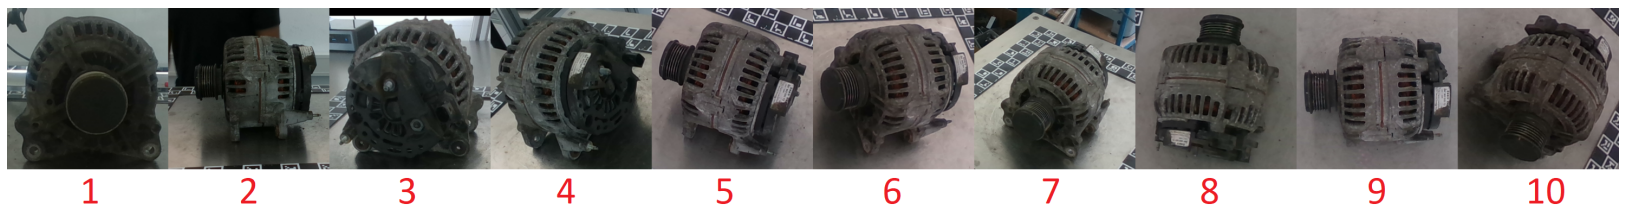
\includegraphics[width=\textwidth]{figure_mvip_ex_cropped_1.png}
	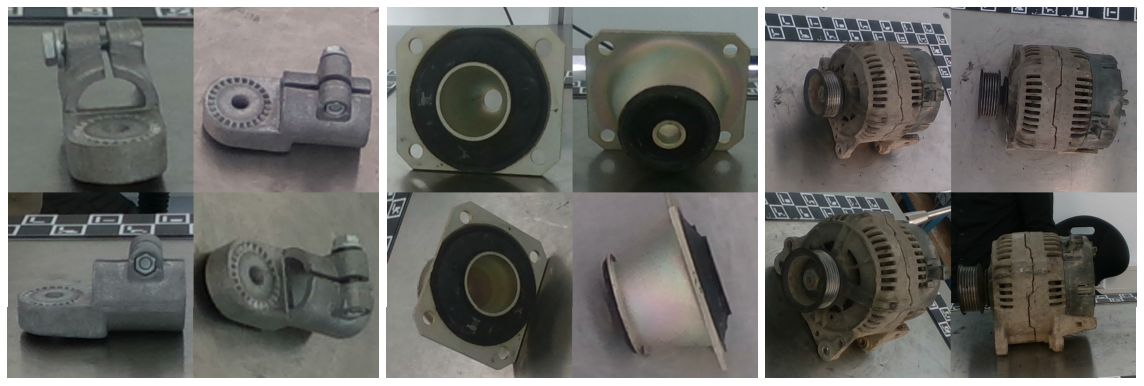
\includegraphics[width=\textwidth]{figure_mvip_ex_cropped_2.png}
	\caption[Beispielbilder aus dem MVIP-Datensatz, die auf die	Region of Interest (ROI) zugeschnitten wurden.]{Beispielbilder aus dem MVIP-Datensatz, die auf die\\
	Region of Interest (ROI) zugeschnitten wurden \parencite{Koch2023mvip}.}
	\label{fig:mvip-examples}
\end{figure}

\subsection{Teildatensatz} \label{sec:subdataset}

% Wahl eines Teildatensatzes mit 20 "CarComponent" Klassen
Da für die Experimente relativ viele Trainings- und Testdurchläufe vorgesehen waren, war es notwendig, einen Teildatensatz auszuwählen, um die Rechenzeit zu reduzieren.

Konkret wurden zufällig 20 Klassen aus der Oberklasse "CarComponent" ausgewählt. Für die Experimente wurden nur die RGB-Bilddaten verwendet, wobei die Segmentierungsmasken in der Vorverarbeitung zum Einsatz kommen (siehe Abschnitt \ref{sec:preprocessing}).

Insgesamt enthält der Teildatensatz ... Bilder. In Tabelle \ref{tab:subdataset} sind die Klassen im Detail aufgeführt.

\begin{table}[]
	%\centering
	\caption{Auswahl der 20 Klassen aus der Oberklasse "CarComponent" für den MVIP-Teildatensatz.}
	\begin{tabular}{|l|l|c|}
		\hline
		\textbf{Klasse} & \textbf{Beschreibungen} & \textbf{Anzahl Bilder} \\
		\hline
		1 ... & ... & ... \\
		2 ... & ... & ... \\
		3 ... & ... & ... \\
		4 ... & ... & ... \\
		5 ... & ... & ... \\
		6 ... & ... & ... \\
		7 ... & ... & ... \\
		8 ... & ... & ... \\
		9 ... & ... & ... \\
		10 ... & ... & ... \\
		11 ... & ... & ... \\
		12 ... & ... & ... \\
		13 ... & ... & ... \\
		14 ... & ... & ... \\
		15 ... & ... & ... \\
		16 ... & ... & ... \\
		17 ... & ... & ... \\
		18 ... & ... & ... \\
		19 ... & ... & ... \\
		20 ... & ... & ... \\
		\hline
	\end{tabular}
	\label{tab:subdataset}
\end{table}

\subsection{Vorverarbeitung} \label{sec:preprocessing}

% Maske -> Bounding Box -> Quadratischer ROI Crop
Die Vorverarbeitung der Bilder unterscheidet sich nur leicht zwischen den beiden Modellen DA-Fusion und Supervised Contrastive Learning. In beiden Fällen werden die Bilder auf die Region of Interest (ROI) zugeschnitten, um den Fokus auf die Objekte zu legen und den Hintergrund zu minimieren. Dazu werden die Segmentierungsmasken verwendet, um die Bounding Box der Objekte zu bestimmen und die Bilder entsprechend zuzuschneiden. Die Ausgabe ist ein quadratisches Bild, das die Objekte in der Mitte enthält.

% "Klassische" Augmentationen; Rotation, ColorJitter, Normalisierung
Zusätzlich werden verschiedene "klassische" Augmentationen angewendet, um die Daten zu erweitern und die Modelle robuster zu machen. Dazu gehören z.B. Rotation, ColorJitter und Normalisierung. Die Parameter für die Augmentationen wurden eher konservativ gewählt, damit die feinen Unterschiede zwischen den Klassen nicht verwischt werden.

\section{Implementierung} \label{sec:implementation}

% Einleitung; Rechner-Zugang, Programmiersprache, Bibliotheken
Zur Vorbereitung und Durchführung der Experimente wurde seitens des Fraunhofer-IPK ein Zugang zu einem leistungsstarken Rechner bereitgestellt, der über zwei NVIDIA-Grafikkarten mit CUDA-Unterstützung\footnote{\textit{Compute Unified Device Architecture}, eine API-Technologie von NVIDIA für parallele Berechnungen auf Grafikkarten} verfügt. Die Implementierung der Modelle und Experimente erfolgte in Python 3.7 unter Verwendung der Bibliotheken PyTorch 1.12.1, Torchvision 0.13.1 und weitere.

% Implementierung von DA-Fusion und Supervised Contrastive Learning
Dabei stützt sich diese Arbeit größtenteils auf die Implementierungen von DA-Fusion aus \parencite{Trabucco2024dafusiongithub} und Supervised Contrastive Learning aus \parencite{Tian2023supcongithub}. Die grundlegende Funktionsweise dieser Implementierungen, sowie die Anpassungen, die im Rahmen des untersuchten Ansatzes vorgenommen wurden, sollen nun genauer erläutert werden.
% Dabei stützt sich diese Arbeit größtenteils auf die Implementierungen von DA-Fusion\footnote{GitHub Repository: \url{https://github.com/brandontrabucco/da-fusion} [Aufgerufen: 16.09.2024]} und Supervised Contrastive Learning\footnote{GitHub Repository: \url{https://github.com/HobbitLong/SupContrast} [Aufgerufen: 16.09.2024]}, die im Rahmen der Forschungsarbeiten von den jeweiligen Autoren entwickelt wurden. Die grundlegende Funktionsweise dieser Implementierungen, sowie die Anpassungen, die im Rahmen des untersuchten Ansatzes vorgenommen wurden, sollen nun genauer erläutert werden.

\subsection{DA-Fusion} \label{sec:da-fusion-implementation}

% Datensatz
Die Implementierung von DA-Fusion kann weitgehend unverändert angewendet werden, um synthetische Daten für den MVIP-Teildatensatz zu generieren. Allerdings musste dieser zunächst als eigene Klasse mit den Methoden \lstinline{get_image_by_idx(idx)} und \lstinline{get_label_by_idx(idx)} implementiert werden (siehe Anhang \ref{code:da-fusion-mvip}). Insbesondere musste die Auswahl der 20 "CarComponent" Klassen sichergestellt werden, wofür die JSON-Dateien der Objekt-Metadaten ausgelesen werden. Anschließend wird über eine Methode das Laden der entsprechenden Bilder und Masken ermöglicht. Der Rest der Klasse entspricht dem Aufbau der anderen Datensatz-Klassen, die in dem Repository zu finden sind.

% Rundown der Anwendung
Mit der implementierten Klasse kann das Skript \lstinline{fine_tune_upstream.py} aufgerufen werden, um mit den entsprechenden Argumenten zur Wahl des Datensatzes und der Hyperparameter (siehe Abschnitt \ref{sec:da-fusion-setup}) Textual Inversion zum Finetuning eines vortrainierten Stable Diffusion-Modells anzuwenden. Dabei werden Text-Prompts verwendet, die zuvor in einer Liste definiert wurden. Für die Experimente wurde die Liste leicht angepasst, vor allem um weniger angemessene Formulierungen wie \lstinline|"a rendering of a {}"| und \lstinline|"a photo of a cool {}"| zu entfernen.

Während des Trainings werden außerdem mit der Funktion \lstinline{log_validation} Validierungsbilder generiert, welche den \lstinline{validation_prompt} verwenden, der als Argument übergeben wird. Diese Bilder sind nicht mit den später generierten Augmentationen vergleichbar, da sie von Grund auf neu generiert werden, bieten aber eine Möglichkeit, den Verlauf des Trainings zu überwachen.

Die gelernten Text-Embeddings werden als .pt-Dateien gespeichert und anschließend mit dem Skript \lstinline{aggregate_embeddings.py} zusammengeführt, um ein klassenagnostisches Template zu erstellen, das im nachfolgenden Schritt verwendet wird.

Um schließlich die Augmentationen zu generieren, wird das Skript \lstinline{generate_augmentations.py} ausgeführt. Hier wird eine Stable Diffusion Image-to-Image-Pipeline\footnote{Die Pipeline verwendet das \textbf{SDEdit}-Framework, das in \parencite{Meng2022sdedit} vorgeschlagen wurde.} verwendet, um den Bildern des Datensatzes Rauschen hinzuzufügen und unter Konditionierung auf den gelernten Text-Embeddings wiederherzustellen. Der genaue Prompt kann als Argument übergeben werden, wobei \lstinline|"a photo of a {}"| als Standardwert verwendet wird. Das \lstinline{strength}-Argument entscheidet, wie viel Rauschen hinzugefügt wird und an welchen Timestep das Bild in das Denoising-Modul eingesetzt wird, wodurch mehr oder weniger stark veränderte Bilder entstehen.

\subsection{Supervised Contrastive Learning} \label{sec:supcon-implementation}

% Kurze Einführung in die bestehende Implementierung
Die Implementierung von Supervised Contrastive Learning verwendet zwei Trainings-Skripte; eins für das Pre-Training der latenten Repräsentationen und eins für die lineare Klassifikation der Repräsentationen.

% Klasse zum Laden des MVIP-Teildatensatzes und der Augmentationen
Zunächst wird die Klasse für den MVIP-Teildatensatz, die für die Implementierung von DA-Fusion verwendet wurde, größtenteils übernommen und in die Trainingsskripte integriert. Die Klasse musste nun allerdings um einige Parameter und Funktionen erweitert werden, um die Verwendung der synthetischen Augmentationen aus DA-Fusion zu konfigurieren (siehe Anhang \ref{code:supcon-mvip}). So steuert der Parameter \lstinline{aug_mode}, ob keine Augmentationen, ausschließlich ID-Augmentationen oder auch die Near OOD-Augmentationen verwendet werden sollen. Über \lstinline{aug_dir_id} und \lstinline{aug_dir_id} werden die Pfade zu den entsprechenden Augmentationen angegeben. Außerdem wurde mit den Parametern \lstinline{aug_ex_id} und \lstinline{aug_ex_ood} eine Einstellung für die Anzahl der verwendeten ID- und OOD-Augmentationen pro Klasse implementiert. % aug_mode = None, "with_id", "with_both", "id_only", "ood_only"

% Pre-Training
Das Pre-Training der latenten Repräsentationen erfolgt mit dem Skript \lstinline{main_supcon.py}, indem ein klassischer Trainingsdurchlauf implementiert wird. Das Modell wird dabei mit einem ResNet-Backbone und einem Projection Head initialisiert. Im Training generiert es die latenten Repräsentationen der Bilder, die dann zusammen mit den Labels in die kontrastive Verlustfunktion gegeben werden. Diese berechnet zunächst eine kontrastive Maske, die die positiven und negativen Paare definiert. Anschließend werden die Kosinus-Ähnlichkeiten der Paare berechnet und die durchschnittliche negative Log-Wahrscheinlichtkeit der positiven Paare als Verlust zurückgegeben.

Für die Experimente dieser Arbeit war die Anpassung dieser Verlustfunktion entscheidend (siehe Anhang \ref{code:supcon-loss}). Dafür wird die kontrastive Maske zunächst so gefiltert, dass keine positiven Paare mit OOD-Daten entstehen, indem diese durch ein negatives Label identifiziert wurden. Nachdem dann die Ähnlichkeitswerte berechnet wurden, werden diese nochmals maskiert, sodass aus den negativen Paaren mit OOD-Daten nur solche übrig bleiben, bei denen die OOD-Augmentation aus der selben Klasse generiert wurde, wie das ID-Bild. Die Verlustfunktion wird dann nur auf diese Paare angewendet.

% Lineare Klassifikation
Das trainierte Modell, welches im Verlauf des Pre-Trainings gespeichert wurde, wird anschließend mit dem Skript \lstinline{main_linear.py} für die lineare Klassifikation verwendet. Dabei wird das Modell mit einem neuen Head initialisiert, der die latenten Repräsentationen in die Klassenlabels überführt. Das Training erfolgt dann mit einer klassischen Cross Entropy-Verlustfunktion, die die Repräsentationen auf die Klassen abbildet.

% Metriken für Evaluation
	% Accuracy
	% ID- und OOD-Confidence

\section{Versuchsaufbau} \label{sec:experiment-setup}

% Einleitung
Die Untersuchung der Forschungsfragen erfolgte in zwei Schritten: Zunächst werden synthetische Daten mit DA-Fusion generiert. Anschließend werden die synthetischen Daten in den Trainings- und Testdurchläufen mit Supervised Contrastive Learning verwendet, um die Auswirkungen der Augmentationen auf die Klassifikation zu evaluieren.

\subsection{Synthetische Datengenerierung} \label{sec:da-fusion-setup}

% ID- & Near OOD-Augmentationen
Es wurden mit DA-Fusion zwei unterschiedliche Sätze von Augmentationen generiert: ID-Augmentationen und Near OOD-Augmentationen.

% Textual Inversion Finetuning:
	% model="CompVis/stable-diffusion-v1-4"
	% initializer_token="motor"
	% num_vectors=16
	% resolution=512
	% examples_per_class=32
	% train_batch_size=16
	% lr=5.0e-04
	% lr_scheduler="constant_with_warmup"
	% lr_warmup_steps=150
	% mixed_precision=fp16
	% max_train_steps=1000
Für beide Sätze wurde das Modell \lstinline{CompVis/stable-diffusion-v1-4}\footnote{Ein vortrainiertes HuggingFace-Modell: \url{https://huggingface.co/CompVis/stable-diffusion-v1-4}} verwendet, das mit dem Token \lstinline{"motor"} initialisiert wurde. Dabei wurden 16 Vektoren pro Token verwendet. Das Finetuning erfolgte mit einer Batch Size von 16, einer Lernrate von 0.0005 und einer konstanten Lernrate mit Warmup über 150 Schritte. Es wurde Mixed Precision mit FP16 verwendet und das Training wurde nach 1000 Schritten beendet. Die erlernten Text-Embeddings wurden für beide Sätze verwendet, um die Augmentationen zu generieren.

% Generierung:
	% aug="real-guidance"
	% guidance_scale=15
	% prompt="a photo of a {}"
	% strength=0.2/0.5
	% examples_per_class=16
	% num_synthetic=4
Die Generierung erfolgte mit der Real Guidance Pipeline und einer Guidance Scale von 15. Es wurden 16 Beispiele pro Klasse zur Augmentation herangezogen und für jedes Beispiel vier synthetische Bilder generiert. Die Segmentierungsmasken wurden verwendet, um die Augmentation auf den Bereich des Objekts zu begrenzen. Die ID- und Near OOD-Augmentationen unterscheiden sich nur durch den \lstinline{strength}-Parameter, wobei für die ID-Augmentationen ein Wert von 0.2 und für die Near OOD-Augmentationen ein Wert von 0.5 verwendet wurde.

\subsection{Trainings- und Testdurchläufe} \label{sec:supcon-setup}

% Drei Versuche; jeweils Contrastive Pre-Training & Lineare Klassifikation
Die Trainings- und Testdurchläufe mit Supervised Contrastive Learning sind in drei Versuchsreihen unterteilt. In jedem Versuch wird zunächst das Pre-Training der latenten Repräsentationen durchgeführt, gefolgt von der linearen Klassifikation der Repräsentationen. Die Versuchsreihen unterscheiden sich in der Verwendung der synthetischen Augmentationen:

\begin{enumerate} %[font=\bfseries]
	\item Nur reale Daten werden verwendet, sowohl für das Pre-Training als auch für das Training des Klassifikators.
	\item Neben den realen Daten werden auch ID-Augmentationen verwendet, sowohl für das Pre-Training als auch für das Training des Klassifikators.
	\item Wie Versuch 2, aber im Pre-Training werden zusätzlich Near OOD-Augmentationen als harte negativ-Beispiele verwendet, wie in Abschnitt \ref{sec:da-fusion-supcon} beschrieben.
\end{enumerate}

% Hyperparameter
Für das Pre-Training wurde eine Batch Size von 16, eine Lernrate von 0.001 mit Kosinus-Annealing und einer Dauer von 110 Epochen verwendet. Die Bilddaten wurden im Rahmen der Augmentation auf eine Größe von 224x224 Pixeln zugeschnitten und normalisiert. Bei der linearen Klassifikation sind die Hyperparameter identisch, jedoch mit einer Dauer von 25 Epochen.

% Evaluierung auf Testdaten
Nach den Trainingsdurchläufen werden die Modelle auf den (echten) Testdaten evaluiert.

\section{Evaluationsmethoden und Metriken} \label{sec:evaluation}

% Menschliche Evaluierung der Augmentationen selbst
Die Qualität der synthetischen Daten, die mit DA-Fusion generiert wurden, werden durch einfache visuelle Inspektion selbst überprüft. Bei den ID-Augmentationen wird darauf geachtet, dass die Objekte in den Bildern in ihrer Form möglichst unverändert bleiben, während die Farben und Texturen variieren können und sollen. Bei den OOD-Augmentationen wird darauf geachtet, dass die Objekte stark genug verändert werden, um nicht mehr als Beispiele für die ID-Klassen erkannt zu werden, während sie gleichzeitig noch genug Ähnlichkeit aufweisen, um herausfordernde negative Beispiele zu sein.

% Accuracy, ID- und OOD-Confidence des SCL Klassifikators
Die Ergebnisse der drei Versuchsreihen werden ausgewertet, indem folgende Metriken beim Test der linearen Klassifikation auf den Testdaten gemessen werden:

\begin{itemize}
	\item \textbf{Top-1 Accuracy}: Der Anteil der korrekt klassifizierten Beispiele.
	\item \textbf{ID-Confidence}: Die durchschnittliche Konfidenz des Klassifikators auf den ID-Daten.
	\item \textbf{OOD-Confidence}: Die durchschnittliche Konfidenz des Klassifikators auf den OOD-Daten.
\end{itemize}